\documentclass{article}
\usepackage{minted}
\usepackage{xcolor}
\usepackage{graphicx}
\graphicspath{{./images/}}
\definecolor{LightGray}{gray}{0.9}
\title{Software Development Week 5}
\author{Nathan Le Brun}
\date{\today}

\begin{document}
    \maketitle
    VSV Id: 107027
    \section[Data Structures]{Data Structures and File Formats}
        \subsection{Difference between Array and Record}
            The difference between an \verb|Array| and a \verb|Record| is that an array usually refers to an indexed array whereas a record usually refers to an associative array
        \subsection{File Formats}
            \subsubsection{CSV File}
                \begin{minted}[breaklines, bgcolor=LightGray]{text}
Draw No, Date, Num1, Num2, Num3, Num4, Num5, SuppNum,
45, 7 Mar 2020,  22,   33,   23,   4,    14,   7,
45, 14 Mar 2020, 34,   35,   23,   12,   18,   31
                \end{minted}
            \subsubsection{XML File}
                \begin{minted}[breaklines, bgcolor=LightGray]{xml}
<?xml version="1.0" encoding="UTF-8"?>
<lottoDraws>
    <Draw>
        <DrawNo>45</DrawNo>
        <Date>7 Mar 2020</Date>
        <Num1>22</Num1>
        <Num2>33</Num2>
        <Num3>23</Num3>
        <Num4>4</Num4>
        <Num5>14</Num5>
        <SuppNum>7</SuppNum>
    </Draw>
    <Draw>
        <DrawNo>46</DrawNo>
        <Date>14 Mar 2020</Date>
        <Num1>34</Num1>
        <Num2>35</Num2>
        <Num3>23</Num3>
        <Num4>12</Num4>
        <Num5>18</Num5>
        <SuppNum>31</SuppNum>
    </Draw>
</lottoDraws>
                \end{minted}
    \section[Iteration]{Iteration (Loops)}
        \subsection{Difference between While and Do While Loop}
             The difference between a \verb|While| loop and a \verb|Do While| loop is that a \verb|While| loop checks for the condition before executing whereas a \verb|Do While| loop checks for the condition after executing
         \subsection{While / Do While Loop}
            \begin{minted}[breaklines, bgcolor=LightGray]{php}
<?php
  $i = 0
  while ($i < 10) {
    $i = $i + 1;
    echo $i;
  }
?>
            \end{minted}
        \subsection{Maximum Temperature}
            \begin{minted}[breaklines, bgcolor=LightGray]{php}
<?php
  $data = array(
    array("12th", "13th", "14th", "15th", "16th", "17th", "18th", "19th", "20th", "21st", "22nd", "23rd", "24th", "25th"),
    array(23.3, 20.8, 20, 24.6, 31.3, 28.8, 31.8, 32.6, 23.8, 20.6, 21.8, 19.2, 20.2, 24.3)
  );
  
  function checkTemp(string $date, float $temp) {
    if ($temp < 20.0 || ($temp > 22.0 && $temp < 32.0)) {
      return "$date: $temp <br>";
    }
  }
  
  for ($i = 0; $i < count($data[0]); $i++) {
    echo checkTemp($data[0][$i], $data[1][$i]);
  }
?>
            \end{minted}
            \begin{figure}[h]
                \centering
                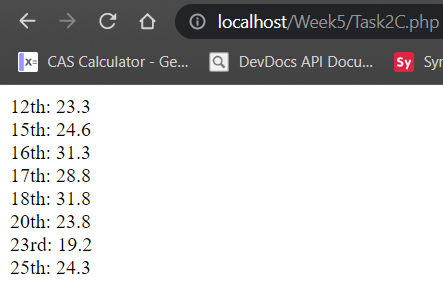
\includegraphics[width=1.0\textwidth]{Task2COutput}
                \caption{The output of the code shown above}
            \end{figure}
\end{document}